\section{Hydrostatic Fluid Pressure}

%Lecture 30, 31, 32
\textbf{Pascal's Law:} A fluid at rest creates a pressure point \textit{p} at a point that is the same in all directions. 

\subsection{Fluid Pressure}

For an incompressible fluid (density $\rho$) at rest, the pressure $p$ varies linearly with fluid depth $z$. This means that the pressure along a horizontal plane (at a certain depth $z$ is constant.

\begin{figure*}[!h]
\centering
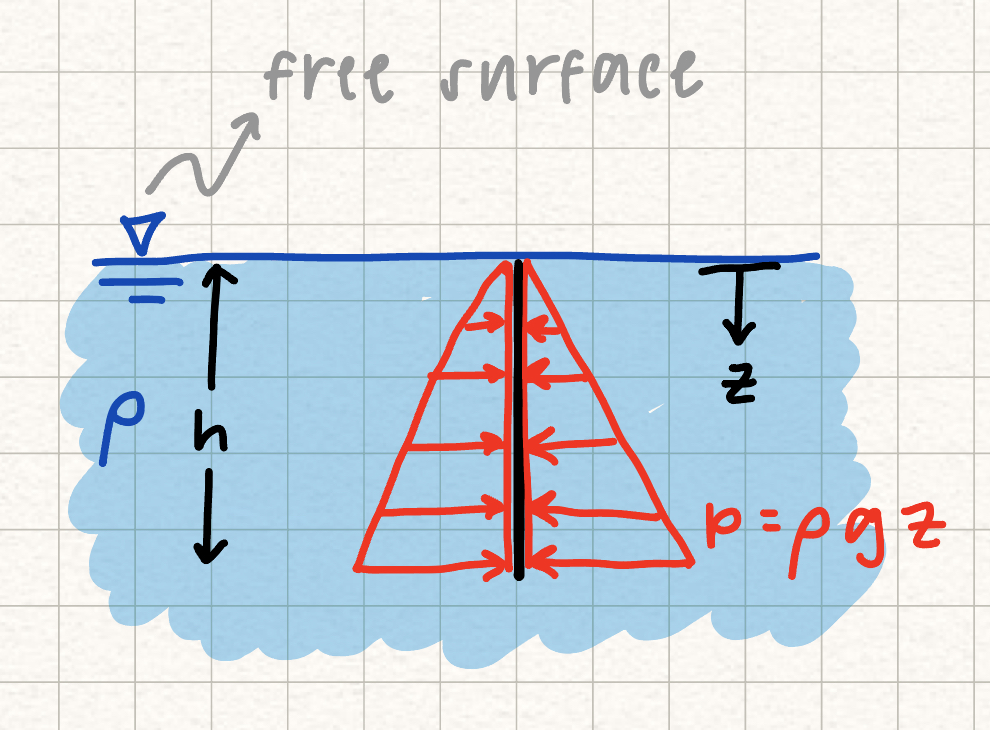
\includegraphics[angle=0, width=4in]{FluidFigures/HydrostaticPressure.jpg}
\vspace{-2mm}
\caption{\small Derivation of the pressure $P(z)$ at the bottom of a cylinder of liquid with cross-sectional area $A$}
\vspace{-3mm}
\label{Fig:HydrostaticPressure}
\end{figure*}

The fluid pressure $P(z)$ can be written as: 

\[P(z) = \rho*g*z\]

\noindent Derivation: 

\begin{figure*}[!h]
\centering
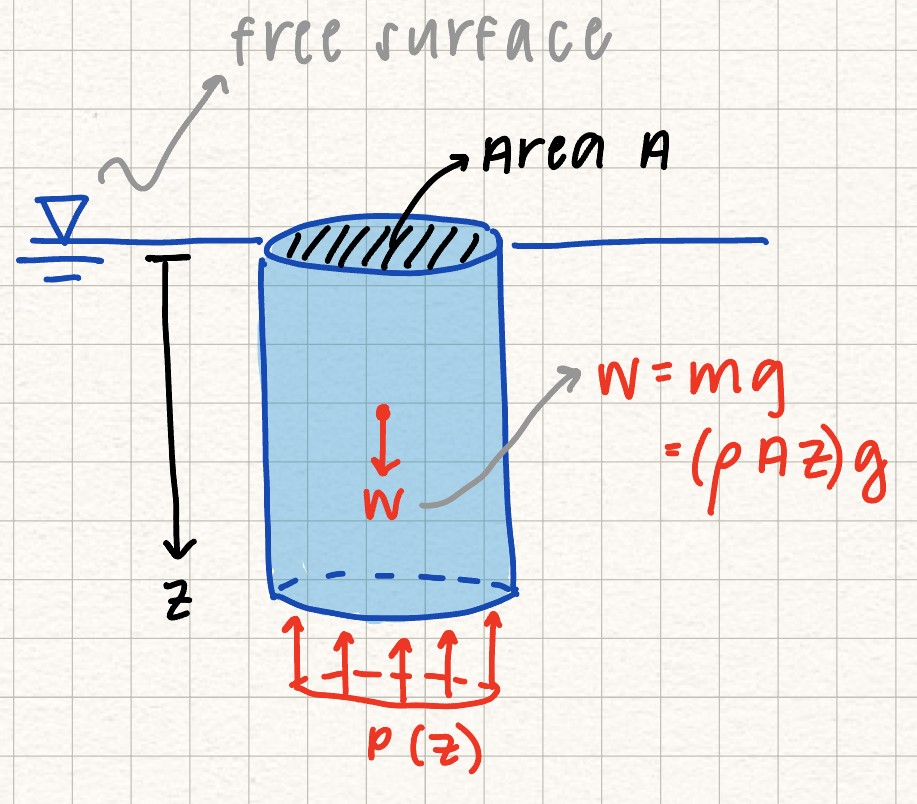
\includegraphics[angle=0, width=\textwidth]{FluidFigures/FluidDerivation.jpg}
\vspace{-2mm}
\caption{\small Derivation of the pressure $P(z)$ at the bottom of a cylinder of liquid with cross-sectional area $A$}
\vspace{-3mm}
\label{Fig:FluidDerivation}
\end{figure*}

\subsection{Buoyancy}

\textbf{Archimedes' Principle:} Any object that is either partially or totally immersed in a fluid has a buoyancy force equal to the weight of the fluid displaced by the object. 


\blue{Do we need to include anything else for buoyancy?}
%Lecture 32